\newpage
\section*{Resultados e Discussão}
\addcontentsline{toc}{chapter}{Resultados e Discussão}

Como referido anteriormente, foram utilizados dois tipos de teste, teste nos dados de treino e teste nos dados de teste. Ambos utilizam 70\% dos dados originais. Mas no caso do teste em dados de teste, 30\% dos dados são utilizados para teste.

Após o ajuste de hiperparâmetros, os melhores resultados obtidos para o teste nos dados de teste foram os seguintes:

\begin{figure}[H]
    \begin{center}
    \setlength{\arrayrulewidth}{0.5mm}
    \renewcommand{\arraystretch}{1.5}
    \begin{tabular}{|c|c|c|c|c|c|}
        \hline
        \textbf{Modelo} & \textbf{AUC} & \textbf{CA} & \textbf{F1} & \textbf{Precision} & \textbf{Recall} \\
        \hline
         Tree  &  0.849 & 0.808 & 0.809 & 0.811 & 0.808 \\
         \hline
         \color{red}{SGD} & 0.904 & 0.857 & 0.857 & 0.857 & 0.857 \\
         \hline
         \color{red}{Random Forest} & 0.920 & 0.847 & 0.847 & 0.850 & 0.847 \\ 
         \hline
         \color{red}{Neural Network} & 0.904 & 0.868 & 0.867 & 0.868 & 0.868 \\
         \hline
         Naive Bayes & 0.895 & 0.812 & 0.812 & 0.815 & 0.812 \\ 
         \hline
         \color{red}{Logistic Regression} & 0.905 & 0.850 & 0.850 & 0.851 & 0.850 \\ 
         \hline
         Gradient Boosting & 0.916 & 0.819 & 0.819 & 0.820 & 0.819 \\ 
         \hline
         AdaBoost & 0.768 & 0.767 & 0.767 & 0.769 & 0.767  \\
         \hline
    \end{tabular}
\end{center}
\selectlanguage{portuguese} \caption{Resultados do Teste em dados de teste}
\end{figure}

Os modelos onde foram obtidos melhores resultados foram "SGD", "Random Forest", "Neural Network" e "Logistic Regression", sendo que o modelo onde se obteve mais precisão foi o "Neural Network". Podemos ainda verficar que "Random Forest" foi o modelo onde "AUC" é mais elevado, apesar da precisão mais baixa.
\newpage

Podemos verificar através do seguinte gráfico uma comparação entre o "ROC" do "Neural Network" e do "Random Forest", estes resultados são para o target "no":


\begin{figure}[H]
    \centering
    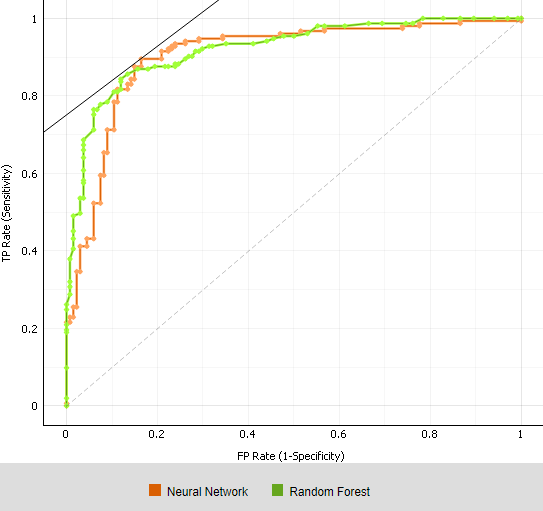
\includegraphics[scale=0.8]{images/roccompare.png}
    \selectlanguage{portuguese} \caption{Comparação de ROC}
\end{figure}

Verificamos através deste gráfico que os resultados do "Random Forest" são melhores para valores de especificidade mais baixos. No entanto são melhores no "Neural Network" para valores mais elevados.


\newpage
Nos resultados do teste nos dados de treino foram obtidos alguns resultados interessantes:

\begin{figure}[H]
\begin{center}
    \setlength{\arrayrulewidth}{0.5mm}
    \renewcommand{\arraystretch}{1.5}
    \begin{tabular}{|c|c|c|c|c|c|}
        \hline
        \textbf{Modelo} & \textbf{AUC} & \textbf{CA} & \textbf{F1} & \textbf{Precision} & \textbf{Recall} \\
        \hline
         Tree  &  0.874 & 0.855 & 0.855 & 0.858 & 0.855 \\
         \hline
         SGD & 0.915 & 0.833 & 0.833 & 0.833 & 0.833 \\
         \hline
         \color{red}{Random Forest} & 1.000 & 1.000 & 1.000 & 1.000 & 1.000 \\ 
         \hline
         Neural Network & 0.912 & 0.832 & 0.832 & 0.832 & 0.832 \\
         \hline
         Naive Bayes & 0.892 & 0.820 & 0.819 & 0.821 & 0.820 \\ 
         \hline
         Logistic Regression & 0.908 & 0.826 & 0.826 & 0.826 & 0.826 \\ 
         \hline
         \color{blue}{Gradient Boosting} & 0.982 & 0.933 & 0.933 & 0.934 & 0.933 \\ 
         \hline
         \color{red}{AdaBoost} & 1.000 & 1.000 & 1.000 & 1.000 & 1.000  \\
         \hline
         
    \end{tabular}
\end{center}
\selectlanguage{portuguese} \caption{Resultados do Teste em dados de treino}
\end{figure}


Podemos verificar que existem dois modelos,"Random Forest" e "AdaBoost", onde os valores são perfeitos. Temos ainda o "Gradient Boost" onde podemos observar valores também elevados.

Estes resultados, quando comparados com os resultados do teste em dados de teste podem parecer invulgares, no entanto, o mais provável é que se trate de \textit{overfitting}. O modelo está demasiado ajustado aos dados de treino o que causa resultados medíocres quando recebe dados diferentes.

Conseguimos ainda verificar outro problema, os modelos, com a exceção dos 3 acima referidos, todos verificam precisões abaixo dos 90\% quando testados com dados de treino, isto leva a querer que a quantidade de dados presente no \textit{dataset} não é suficiente para treinar o modelo de forma eficiente.

Com isto tiramos duas conclusões, os modelos que apresentam precisão superior a 90\% nos dados de treino apresentam \textit{overfitting} e os restantes não têm dados suficientes para fazer um bom treino do modelo.






